\documentclass[border=0cm]{standalone}
\usepackage{xcolor}
\usepackage{tikz}
\usetikzlibrary{arrows, arrows.meta}
\definecolor{light-gray}{gray}{0.975}
\definecolor{pcolor}{rgb}{0.21, 0.27, 0.31}
\definecolor{purple}{rgb}{1.0, 0.0 0.0}
\definecolor{pgreen}{rgb}{0.0, 0.5 0.0}
\tikzset{
    barbarrow/.style={ % style that just defines the arrow tip
        >={Straight Barb[left,length=5pt,width=5pt]},
        thick,
        <->
    },
    blues/.style={
        color=blue
    },
    reds/.style={
        color=pgreen
    }
}
\begin{document}
\begin{tabular}{c c c c c}
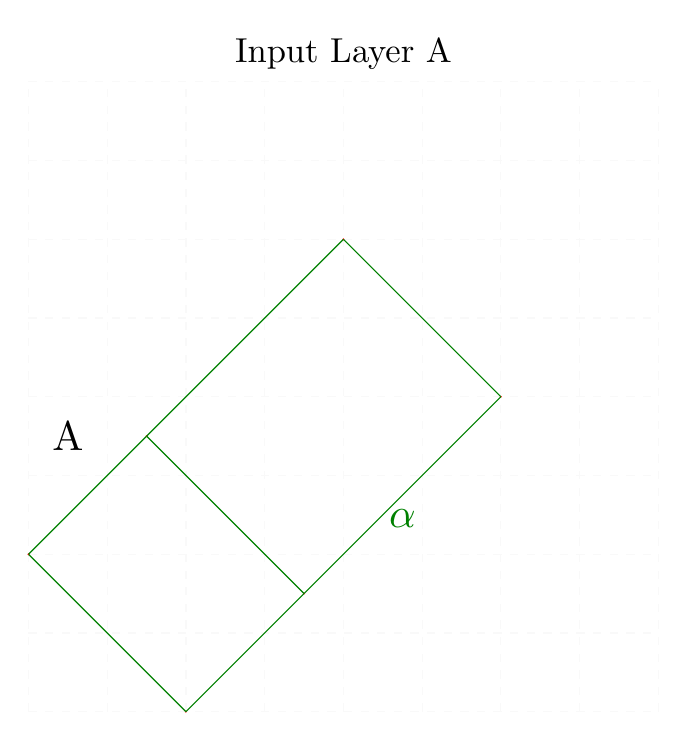
\begin{tikzpicture}
    \tikzstyle{node1}=[draw,scale=0.02,shape=circle,color=red,fill=red]
    \draw[color=light-gray, style=dashed] (0,0) grid (8,8);

    \node[above, scale=1.25] at (4,8) {Input Layer A};
    \node[node1] (A)  at (0,2) {};
    \node[node1] (C)  at (2,0) {};
    \node[node1] (E)  at (1.5,3.5) {};
    \node[node1] (K)  at (3.5,1.5) {};
    \node[node1] (M) at (4,6)  {};
    \node[node1] (R)  at (6,4) {};
    \node[scale=1.5] at (0.5,3.5) {A};

    \draw[reds](A) -- (C);\draw[reds](A) -- (E);
    \draw[reds](C) -- (K);\draw[reds](E) -- (K);
    \draw[reds](E) -- (M);\draw[reds](K) -- (R) node[midway, below,scale=1.5] {$\alpha$};
    \draw[reds](M) -- (R);
\end{tikzpicture} 
&
\begin{tikzpicture}
    \draw[color=white, style=dashed] (0,0) grid (0,8);
    \node[scale=4] at (0, 4) {$\Longrightarrow$};
\end{tikzpicture} 
&
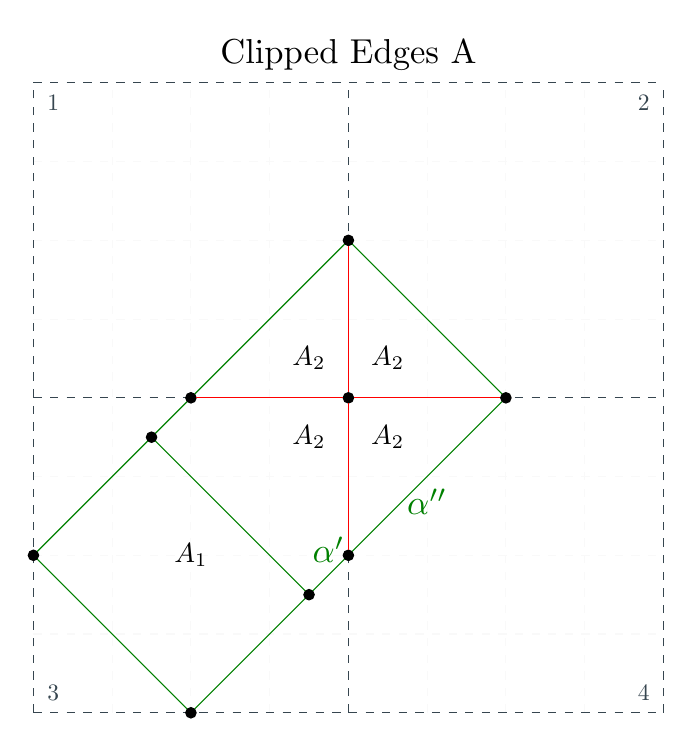
\begin{tikzpicture}
    \tikzstyle{node1}=[draw,scale=0.4,shape=circle,color=black,fill=black]
    \tikzstyle{node2}=[draw,scale=0.4,shape=circle,color=red,fill=red]
    \tikzstyle{text}=[draw,scale=0.5,color=black]
    \draw[color=light-gray, style=dashed] (0,0) grid (8,8);
    \draw[color=pcolor, style=dashed, step=4] (0,0) grid (8,8);
    \node[scale=0.85, color = pcolor] at (0.25, 7.75) {$1$};
    \node[scale=0.85, color = pcolor] at (7.75, 7.75) {$2$};
    \node[scale=0.85, color = pcolor] at (0.25, 0.25) {$3$};
    \node[scale=0.85, color = pcolor] at (7.75, 0.25) {$4$};
    
    \node[above, scale=1.25, thick] at (4,8) {Clipped Edges A};
    \node[node1] (A)  at (0,2) {};
    \node[node1] (C)  at (2,0) {};
    \node[node1] (E)  at (2,4) {};
    \node[node1] (K)  at (4,2) {};
    \node[node1] (M) at (4,6)  {};
    \node[node1] (R)  at (6,4) {};
    \node[node1] (Z)  at (4,4) {};
    \node[node1] (B)  at (1.5,3.5) {};
    \node[node1] (D)  at (3.5,1.5) {};
    \node at (2,2) {$A_1$};
    \node at (3.5,4.5) {$A_2$};
    \node at (4.5,4.5) {$A_2$};
    \node at (3.5,3.5) {$A_2$};
    \node at (4.5,3.5) {$A_2$};
    
    \draw[reds](A) -- (C);
    \draw[reds](A) -- (B);
    \draw[reds](B) -- (E);
    \draw[reds](D) -- (K) node[midway, above,scale=1.25] {$\alpha^{\prime}$};
    \draw[reds](C) -- (D);
    \draw[reds](B) -- (D);
    \draw[reds](E) -- (M);
    \draw[reds](K) -- (R) node[midway, below,scale=1.25] {$\alpha^{\prime \prime}$};
    \draw[reds](M) -- (R);
    \draw[color=purple] (Z) -- (E);
    \draw[color=purple] (Z) -- (R);
    \draw[color=purple] (Z) -- (M);
    \draw[color=purple] (Z) -- (K);
\end{tikzpicture}
&
\begin{tikzpicture}
    \draw[color=white, style=dashed] (0,0) grid (0,8);
    \node[scale=4] at (0, 4) {$\Longrightarrow$};
\end{tikzpicture} 
&
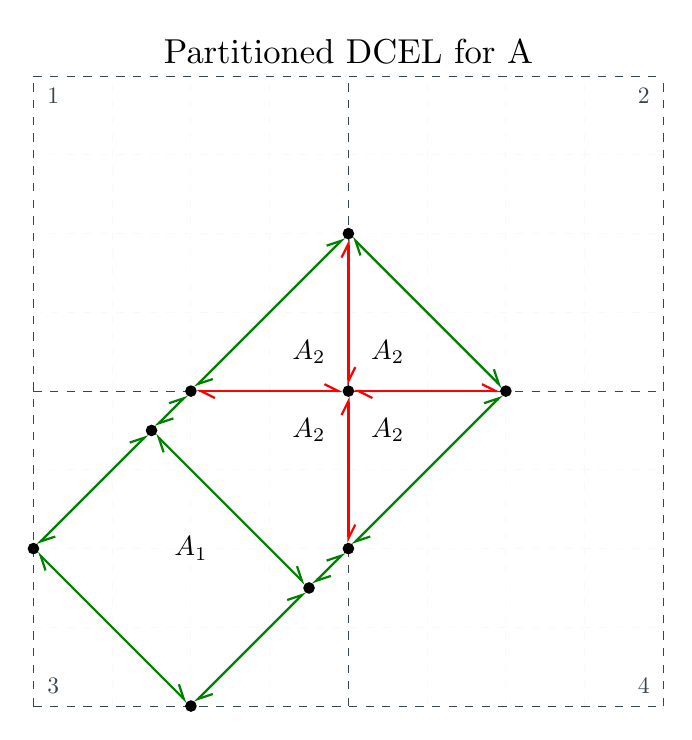
\begin{tikzpicture}
    \tikzstyle{node1}=[draw,scale=0.4,shape=circle,color=black,fill=black]
    \tikzstyle{node2}=[draw,scale=0.4,shape=circle,color=red,fill=red]
    \tikzstyle{text}=[draw,scale=0.5,color=black]
    \draw[color=light-gray, style=dashed] (0,0) grid (8,8);
    \draw[color=pcolor, style=dashed, step=4] (0,0) grid (8,8);
    \node[scale=0.85, color = pcolor] at (0.25, 7.75) {$1$};
    \node[scale=0.85, color = pcolor] at (7.75, 7.75) {$2$};
    \node[scale=0.85, color = pcolor] at (0.25, 0.25) {$3$};
    \node[scale=0.85, color = pcolor] at (7.75, 0.25) {$4$};

    \node[above, scale=1.25, thick] at (4,8) {Partitioned DCEL for A};
    \node[node1] (A) at (0,2) {};
    \node[node1] (C) at (2,0) {};
    \node[node1] (E) at (2,4) {};
    \node[node1] (K) at (4,2) {};
    \node[node1] (M) at (4,6) {};
    \node[node1] (R) at (6,4) {};
    \node[node1] (Z) at (4,4) {};
    \node[node1] (B)  at (1.5,3.5) {};
    \node[node1] (D)  at (3.5,1.5) {};
    \node at (2,2) {$A_1$};
    \node at (3.5,4.5) {$A_2$};
    \node at (4.5,4.5) {$A_2$};
    \node at (3.5,3.5) {$A_2$};
    \node at (4.5,3.5) {$A_2$};
    
    \draw[barbarrow, color=pgreen](A) -- (B);
    \draw[barbarrow, color=pgreen](B) -- (E);
    \draw[barbarrow, color=pgreen](D) -- (K);
    \draw[barbarrow, color=pgreen](C) -- (D);
    \draw[barbarrow, color=pgreen](B) -- (D);

    \draw[barbarrow, color=pgreen] (A) -- (C);
    %\draw[barbarrow, color=pgreen] (A) -- (E);
    %\draw[barbarrow, color=pgreen] (C) -- (K);
    %\draw[barbarrow, color=pgreen] (E) -- (K);
    \draw[barbarrow, color=pgreen] (E) -- (M);
    \draw[barbarrow, color=pgreen] (K) -- (R);
    \draw[barbarrow, color=pgreen] (M) -- (R);
    \draw[barbarrow, color=purple] (Z) -- (E);
    \draw[barbarrow, color=purple] (Z) -- (R);
    \draw[barbarrow, color=purple] (Z) -- (M);
    \draw[barbarrow, color=purple] (Z) -- (K);
\end{tikzpicture}
\\
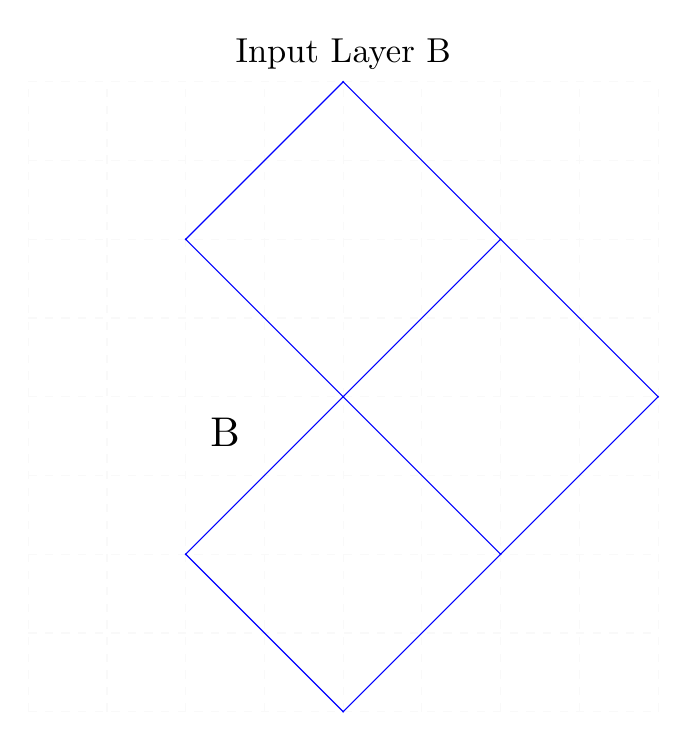
\begin{tikzpicture}
    \tikzstyle{node1}=[draw,scale=0.02,shape=circle,color=blue,fill=blue]
    \draw[color=light-gray, style=dashed] (0,0) grid (8,8);
    \node[above, scale=1.25] at (4,8) {Input Layer B};
    \node[node1] (D) at (2,2) {};
    \node[node1] (F) at (2,6) {};
    \node[node1] (J) at (4,0) {};
    \node[node1] (L) at (4,4) {};
    \node[node1] (N) at (4,8) {};
    \node[node1] (Q) at (6,2) {};
    \node[node1] (S) at (6,6) {};
    \node[node1] (T) at (8,4) {};
    \node[scale=1.5] at (2.5,3.55) {B};

    \draw[blues]
        (D) -- (J) (D) -- (L) (F) -- (N) (F) -- (L) (J) -- (Q)
        (L) -- (Q) (L) -- (S) (N) -- (S) (Q) -- (T) (S) -- (T);
\end{tikzpicture}
&
\begin{tikzpicture}
    \draw[color=white, style=dashed] (0,0) grid (0,8);
    \node[scale=4] at (0, 4) {$\Longrightarrow$};
\end{tikzpicture}
&
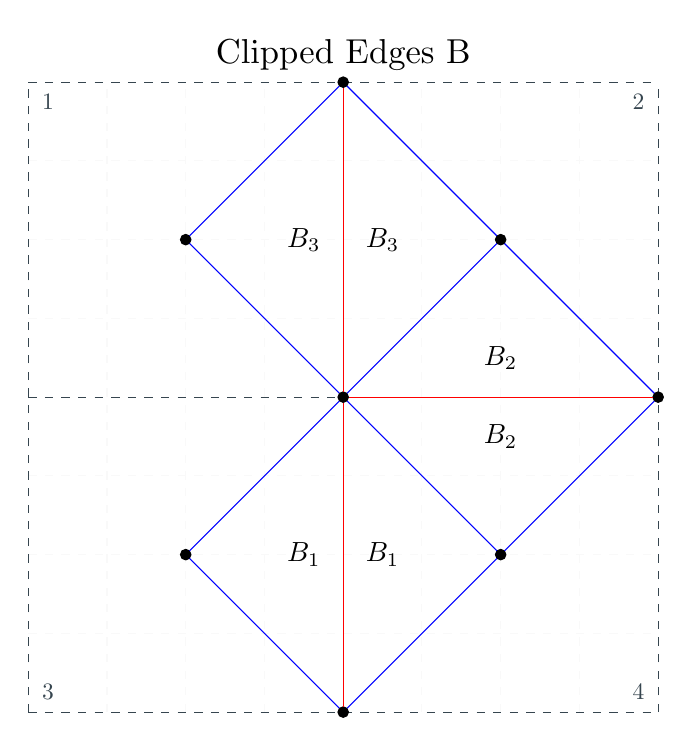
\begin{tikzpicture}
    \tikzstyle{node1}=[draw,scale=0.4,shape=circle,color=black,fill=black]
    \tikzstyle{node2}=[draw,scale=0.4,shape=circle,color=red,fill=red]
    \draw[color=light-gray, style=dashed] (0,0) grid (8,8);
    \draw[color=pcolor, style=dashed, step=4] (0,0) grid (8,8);
    \node[scale=0.85, color = pcolor] at (0.25, 7.75) {$1$};
    \node[scale=0.85, color = pcolor] at (7.75, 7.75) {$2$};
    \node[scale=0.85, color = pcolor] at (0.25, 0.25) {$3$};
    \node[scale=0.85, color = pcolor] at (7.75, 0.25) {$4$};

    \node[above, scale=1.25] at (4,8) {Clipped Edges B};
    \node[node1] (D) at (2,2) {};
    \node[node1] (F) at (2,6) {};
    \node[node1] (J) at (4,0) {};
    \node[node1] (L) at (4,4) {};
    \node[node1] (N) at (4,8) {};
    \node[node1] (Q) at (6,2) {};
    \node[node1] (S) at (6,6) {};
    \node[node1] (T) at (8,4) {};
    \node at (3.5,2) {$B_1$};
    \node at (6,4.5) {$B_2$};
    \node at (3.5,6) {$B_3$};
    \node at (4.5,2) {$B_1$};
    \node at (6,3.5) {$B_2$};
    \node at (4.5,6) {$B_3$};

    \draw[blues](D) -- (J); \draw[blues](D) -- (L);
    \draw[blues](F) -- (N); \draw[blues](F) -- (L);
    \draw[blues](J) -- (Q); \draw[blues](L) -- (Q);
    \draw[blues](L) -- (S); \draw[blues](N) -- (S);
    \draw[blues](Q) -- (T); \draw[blues](S) -- (T);
    \draw[color=purple] (L) -- (T);
    \draw[color=purple] (L) -- (N);
    \draw[color=purple] (L) -- (J);
\end{tikzpicture}
&
\begin{tikzpicture}
    \draw[color=white, style=dashed] (0,0) grid (0,8);
    \node[scale=4] at (0, 4) {$\Longrightarrow$};
\end{tikzpicture}
&
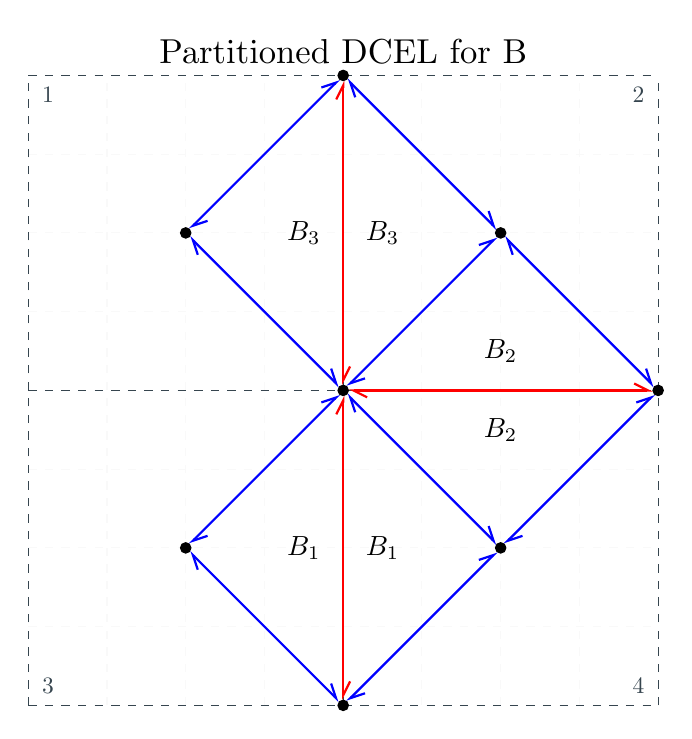
\begin{tikzpicture}
    \tikzstyle{node1}=[draw,scale=0.4,shape=circle,color=black,fill=black]
    \tikzstyle{node2}=[draw,scale=0.4,shape=circle,color=red,fill=red]
    \draw[color=light-gray, style=dashed] (0,0) grid (8,8);
    \draw[color=pcolor, style=dashed, step=4] (0,0) grid (8,8);
    \node[scale=0.85, color = pcolor] at (0.25, 7.75) {$1$};
    \node[scale=0.85, color = pcolor] at (7.75, 7.75) {$2$};
    \node[scale=0.85, color = pcolor] at (0.25, 0.25) {$3$};
    \node[scale=0.85, color = pcolor] at (7.75, 0.25) {$4$};

    \node[above, scale=1.25] at (4,8) {Partitioned DCEL for B};
    \node[node1] (D) at (2,2) {};
    \node[node1] (F) at (2,6) {};
    \node[node1] (J) at (4,0) {};
    \node[node1] (L) at (4,4) {};
    \node[node1] (N) at (4,8) {};
    \node[node1] (Q) at (6,2) {};
    \node[node1] (S) at (6,6) {};
    \node[node1] (T) at (8,4) {};
    \node at (3.5,2) {$B_1$};
    \node at (6,4.5) {$B_2$};
    \node at (3.5,6) {$B_3$};
    \node at (4.5,2) {$B_1$};
    \node at (6,3.5) {$B_2$};
    \node at (4.5,6) {$B_3$};

    \draw[barbarrow, color=blue](D) -- (J);  \draw[barbarrow, color=blue](D) -- (L);
    \draw[barbarrow, color=blue](F) -- (N); \draw[barbarrow, color=blue](F) -- (L);
    \draw[barbarrow, color=blue](J) -- (Q);  \draw[barbarrow, color=blue](L) -- (Q);
    \draw[barbarrow, color=blue](L) -- (S);  \draw[barbarrow, color=blue](N) -- (S);
    \draw[barbarrow, color=blue](Q) -- (T); \draw[barbarrow, color=blue](S) -- (T);
    \draw[barbarrow, color=purple] (L) -- (T);
    \draw[barbarrow, color=purple] (L) -- (N);
    \draw[barbarrow, color=purple] (L) -- (J);
\end{tikzpicture}
\\
\end{tabular}
\end{document}
